\PassOptionsToPackage{table}{xcolor}
\documentclass[12pt,letterpaper,twocolumn,openany,nodeprecatedcode,bg=none]{dndbook}
\usepackage[english]{babel}
\usepackage[utf8]{inputenc}
\usepackage{longtable,booktabs,array}
\usepackage{calc}
\usepackage{etoolbox}
\usepackage{caption}
\usepackage{float}
\usepackage{graphicx}
\usepackage{needspace}
\usepackage{tikz}

% Reset zebra striping at the start of every table
\AtBeginEnvironment{longtable}{\rowcolors{1}{white}{gray!10}\small}
\AtBeginEnvironment{table}{\rowcolors{1}{white}{gray!10}}

\providecommand{\pandocbounded}[1]{#1}
\providecommand{\tightlist}{%
  \setlength{\itemsep}{0pt}\setlength{\parskip}{0pt}}

\captionsetup{labelformat=empty}
\setcounter{secnumdepth}{0}
\setlength{\parindent}{0pt}
\setlength{\parskip}{0.5\baselineskip}
\setlength{\headheight}{15pt}

% Prevent orphaned subsections
\let\oldsubsection\subsection
\renewcommand{\subsection}[1]{%
  \needspace{5\baselineskip}%
  \oldsubsection{#1}%
}

\begin{document}
\onecolumn

      \title{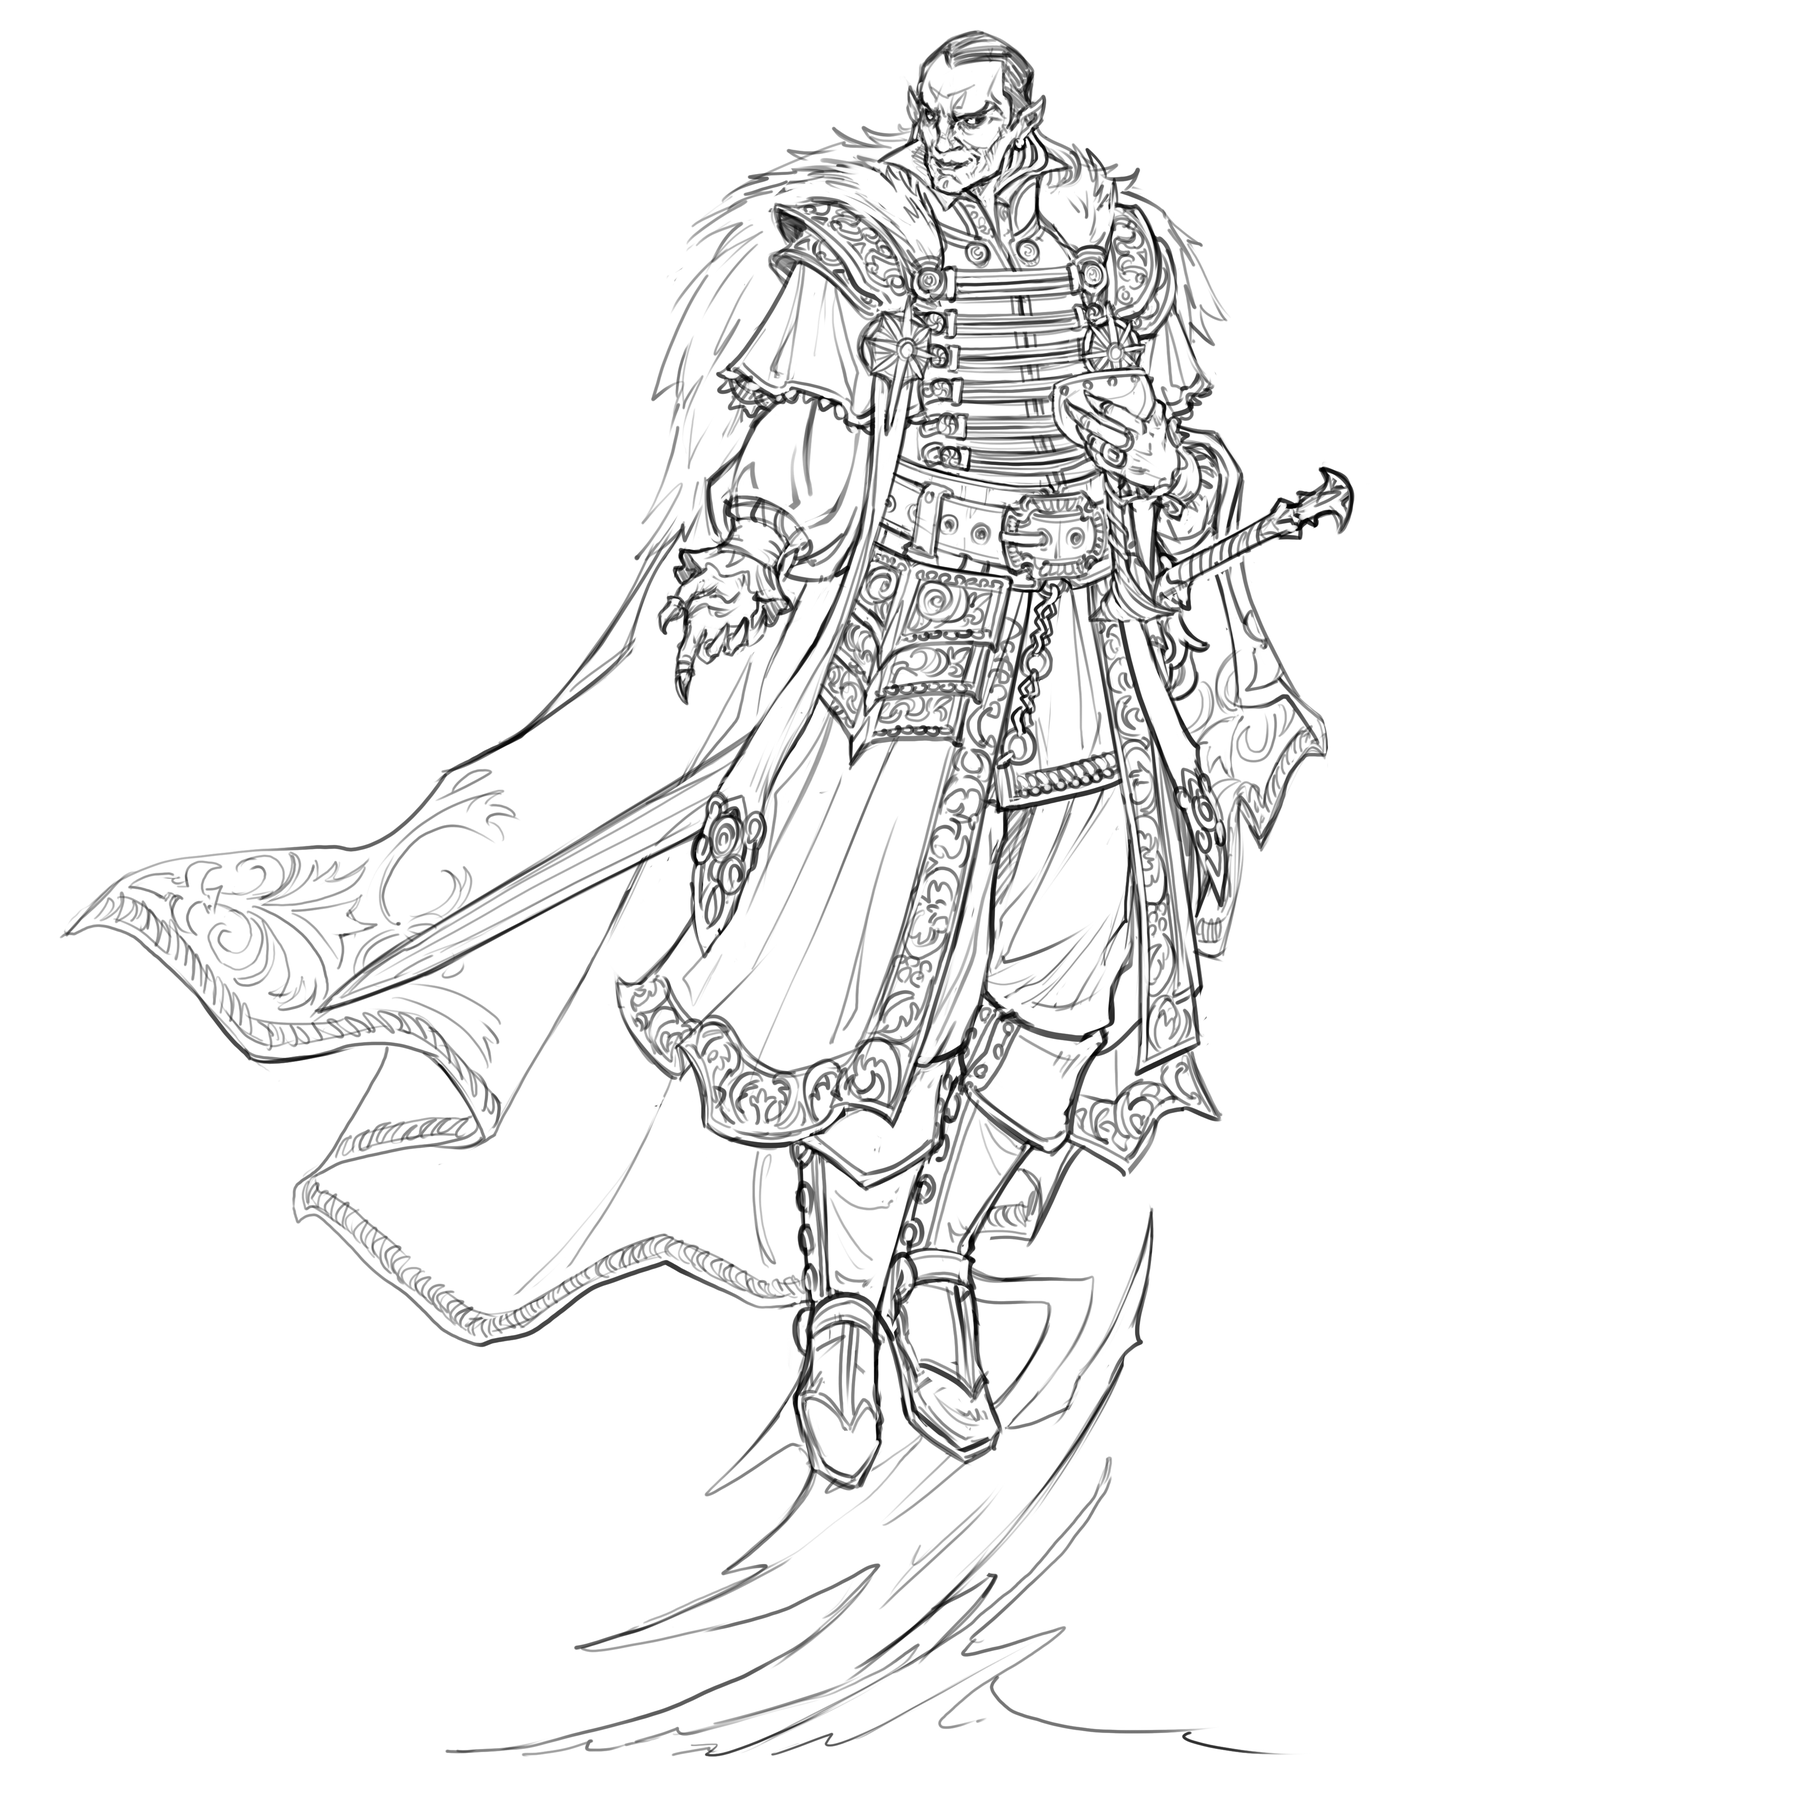
\includegraphics[width=0.9\textwidth,height=0.55\textheight,keepaspectratio]{vampireOC.png}\\[1.5cm]Warlock}
  \author{Class Handbook}
\date{}
\maketitle

\clearpage
\thispagestyle{empty}
\null\vfill
\begin{center}{\Large\itshape Your trusty class handbook for fantasy
gaming.}\end{center}
\vfill

\clearpage
\thispagestyle{empty}
\begin{center}
\vspace*{\fill}
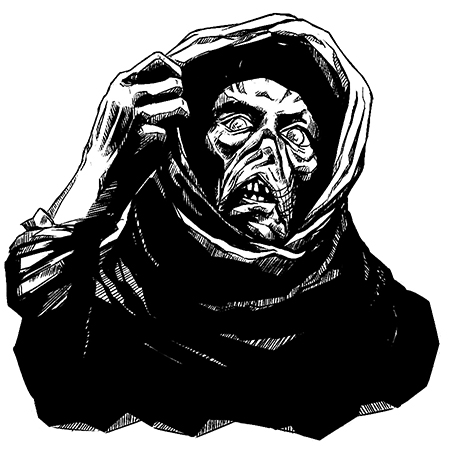
\includegraphics[width=\textwidth,height=0.85\textheight,keepaspectratio]{warlockDisease.jpg}\par
\vspace{0.4cm}
{\itshape With unknown power comes unknown costs}\par
\vspace*{\fill}
\end{center}

\clearpage
\twocolumn

\section{Warlock}\label{warlock}

\subsection{Core Warlock Traits}\label{core-warlock-traits}

\needspace{11\baselineskip}

{\def\LTcaptype{none} % do not increment counter
\begin{table}[!htbp]
\centering
\begin{tabular}{@{}
  >{\raggedright\arraybackslash}p{(\linewidth - 2\tabcolsep) * \real{0.4127}}
  >{\raggedright\arraybackslash}p{(\linewidth - 2\tabcolsep) * \real{0.5873}}@{}}
\toprule\noalign{}
\begin{minipage}[b]{\linewidth}\raggedright
\textbf{Primary Ability}
\end{minipage} & \begin{minipage}[b]{\linewidth}\raggedright
Varies
\end{minipage} \\
\midrule\noalign{}
\textbf{Hit Points} & 1d6 \\
\textbf{Saving Throw Proficiencies} & Intelligence, Wisdom \\
\textbf{Skill Proficiencies} & Choose 4 skills \\
\textbf{Weapon Proficiencies} & Choose 2 categories \\
\textbf{Starting Equipment} & Padded Jacket, Grimoire, Robe, Dagger \\
\bottomrule\noalign{}
\end{tabular}
\end{table}
}

\subsection{Warlock Features}\label{warlock-features}

\needspace{20\baselineskip}

{\def\LTcaptype{none} % do not increment counter
\begin{table}[!htbp]
\centering
\begin{tabular}{@{}
  >{\raggedright\arraybackslash}p{(\linewidth - 4\tabcolsep) * \real{0.1667}}
  >{\raggedright\arraybackslash}p{(\linewidth - 4\tabcolsep) * \real{0.3667}}
  >{\raggedright\arraybackslash}p{(\linewidth - 4\tabcolsep) * \real{0.4667}}@{}}
\toprule\noalign{}
\begin{minipage}[b]{\linewidth}\raggedright
Level
\end{minipage} & \begin{minipage}[b]{\linewidth}\raggedright
Proficiency
\end{minipage} & \begin{minipage}[b]{\linewidth}\raggedright
Class Features
\end{minipage} \\
\midrule\noalign{}
1 & +2 & Warlock Pact \\
2 & +2 & --- \\
3 & +2 & Ability Bonus \\
4 & +2 & --- \\
5 & +2 & --- \\
6 & +2 & --- \\
7 & +2 & Ability Bonus \\
8 & +2 & --- \\
9 & +3 & --- \\
10 & +3 & --- \\
\bottomrule\noalign{}
\end{tabular}
\end{table}
}

\subsection{Level 1: Warlock Pact}\label{level-1-warlock-pact}

You have through either ritual, pact, or sheer force of will, gleamed a
power from a supernatural entity that is beyond mortal comprehension.
Choose one of the pacts listed at the end of this class description
which will grant you your eldritch powers. Your primary ability is
determined by your pact.

Your attack rolls for pact features is equal to your proficiency plus
your primary ability. Your save DC for your pact features is equal to 8
+ proficiency bonus + primary ability.

\subsection{Level 3: Ability Bonus}\label{level-3-ability-bonus}

You gain a +1 bonus to two different abilities of your choice.

\subsection{Level 7: Ability Bonus}\label{level-7-ability-bonus}

You gain a +1 bonus to two different abilities of your choice.

\clearpage

\section{Warlock Pacts}\label{warlock-pacts}

\subsection{Great Old One}\label{great-old-one}

A mysterious entity whose nature is utterly foreign and beyond the very
fabric of reality. You gain the following abilities which you can use at
will.

\textbf{Primary Ability: Intelligence}

\textbf{Level 1: Mind Spike.} Choose a target within 30 feet, they must
make an Intelligence save or take 1d6 psychic damage per warlock level.

\textbf{Level 1: Awakened Mind.} You can telepathically speak to any
creature you can see within 30 feet of you regardless of whether you
share any languages.

\textbf{Level 5: Detect Thoughts.} You sense the presence of thoughts
within 30 feet that belong to creatures that know languages or are
telepathic.

You don't read the thoughts, but you know that a thinking creature is
present.

If you can see a creature, as an action or when you cast this spell you
can force it to make a Wisdom save. If it fails, you search its thoughts
and learn the answer to one question you ask it. You learn the truth as
the creature understands it.

\textbf{Level 5: Thought Shield.} All creatures within 30 feet of you
must make an Intelligence save or take 1d6 psychic damage and cannot
move until the start of your next turn.

\textbf{Level 9: Mind Stun.} All creatures within 30 feet of you must
make an Intelligence save or take 1d6 psychic damage and cannot move
until the start of your next turn.

\textbf{Level 9: Telekinesis.} You can try to move a Huge or smaller
creature or similar size object. Make an ability check with your primary
ability contested by the creature's Strength check, objects fail
automatically. If you succeed, you can move the creature up to 30 feet
in any direction. Until the end of your next turn, a creature who fails
their save is also restrained. Reminder: Creatures take 1d6 bludgeoning
damage for every 10 feet they fall.

\clearpage

\subsection{Undying One}\label{undying-one}

An entity of great necromantic power and unnaturally long life who holds
secrets of the world innumerable and utterly profane.

\textbf{Primary Ability: Wisdom}

\textbf{Level 1: Death's Touch.} Make a melee attack using your primary
ability against a target within 10 feet. They take 1d8 necrotic damage
per warlock level.

\textbf{Level 1: False Life.} Once on your turn, you can regain 1 hit
point by siphoning energy from another living creature within 5 feet of
you. They lose 1 hit point.

\textbf{Level 5: Necromantic Ritual.} You summon a cursed spirit to aid
you in combat. The spirit has the following statistics.

\begin{quote}
\textbf{AC} 13 --- \textbf{HP} 15 --- \textbf{Tests} +1 (Cha +4) --- 40
feet (Fly)

\textbf{Incorporeal.} Can move through but cannot end a turn inside a
solid object.

\textbf{Insubstantial (16+).} The first time this creature takes damage
on a turn, roll a d20. On 16+ it takes no damage that turn.

\textbf{Initiative 10: Necrotic Aura.} Hostile creatures in melee range
must make a Constitution save using the warlock's save DC.
\textbf{Failure:} 1d4 necrotic damage per 2 warlock levels, and
frightened of the spirit for 1 round. \textbf{Success:} Half damage
\end{quote}

\textbf{Level 5: Ray of Sickness.} One target you can see within 60 feet
must make a Constitution save. On a failure, they take 2d10 necrotic
damage and have disadvantage on all rolls until the end of your next
turn.

\textbf{Level 9: Ritual of the Vampire.} You undergo the death ritual to
become a vampire, dying in a coffin and being reborn in blood. You no
longer require food, water, or sleep. Instead, you must consume the
blood of a living or recently dead humanoid creature.

In return, you gain resistance to damage from non-magical weapons,
resistance to cold damage, +2 to all ability scores, bypassing the
normal maximum of +5. When you would die from reaching 3 death save
failures, you do not die unless you take radiant damage, are in
sunlight, or are killed in your coffin. Instead, you turn into mist and
return to the coffin where you performed the ritual of the vampire.

As a cost, you are vulnerable to radiant damage, fire damage, and damage
from silvered weapons. While in direct sunlight, you take 5 radiant
damage at the start of your turn (doubled to 10). A hooded cloak can be
worn to avoid this effect in normal daylight.

\textbf{Level 9: Saving Throws.} You gain proficiency with Strength,
Dexterity, Constitution, and Charisma saves. If you already have
proficiency with these saves, you instead gain expertise with them.

\clearpage

\subsection{Cryptid}\label{cryptid}

This entity is an evil and malevolent creature. A bedtime story told to
children to discourage them from going out into the dark woods. Except
these dark creatures and the mythical powers they say to wield are not
always as fake as they may seem. Sometimes, there really is a monster
under your bed, outside your window, or watching you from behind that
tree\ldots{}

\textbf{Primary Ability: Constitution}

\textbf{Level 1: Curse of Lycanthropy.} Under the cover of darkness, you
transform into a werewolf, or similar hybrid perversion of nature. You
gain an insatiable bloodlust for the hearts of humanoid creatures. If
you do not consume a heart by sunrise, you take a death save failure.

While transformed, you gain a +3 to your Strength, Dexterity, and
Constitution, bypassing the normal maximum of +5. Your unarmed strikes
deal a base 2d6 damage. You also have resistance to bludgeoning,
piercing, and slashing damage, unless it is coming from a silvered
weapon, or more powerful magic weapon.

\textbf{Level 1: Beast Sense.} While transformed or not transformed, you
have advantage on perception checks, and your sense of hearing, smell,
and sight are unmatched. You cannot be surprised and have blindsight out
to 30 feet.

\textbf{Level 1: Saving Throws.} You gain proficiency with Strength,
Dexterity, and Constitution saves. If you already have proficiency with
these saves, you instead gain expertise with them.

\textbf{Level 5: Bloodthirsty Lycanthrope.} You can transform into a
werewolf at will. If it is daylight, this transformation lasts only 1
hour and you take a death save failure if it ends without you consuming
a humanoid heart.

\textbf{Level 5: Extra Attack.} When you attack, you can make two
unarmed attacks.

\textbf{Level 9: Elder Lycanthrope.} You are a master of the rituals of
the hunt and know how to convert others to become a lycanthrope by
sharing in the beast blood ritual. You can grant the Curse of
Lycanthropy and Beast Sense to creatures using this ability. Once cursed
in this way, you do not know how to lift the curse from a creature.

\textbf{Level 9: Extra Attack.} When you attack, you can make three
unarmed attacks.

\onecolumn

\clearpage
\thispagestyle{empty}
\begin{center}
\vspace*{\fill}
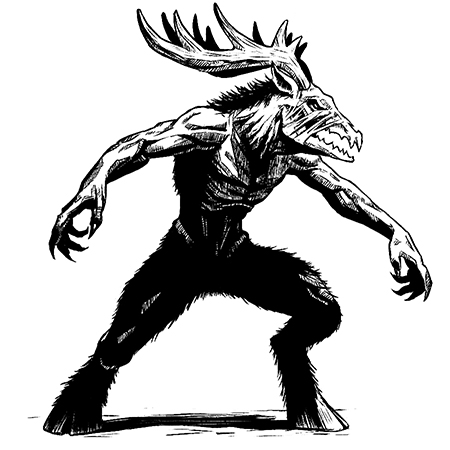
\includegraphics[width=0.7\textwidth,keepaspectratio]{werebeast.jpg}\par
\vspace{0.4cm}
{\itshape What is the worth of single mortal soul?}\par
\vspace*{\fill}
\end{center}

\end{document}